What can you make with 10 different Scratch-blocks?\\
In Figur~\ref{fig:blokke} is shown 10 Scratch-blocks.
\begin{figure}
  \centering
  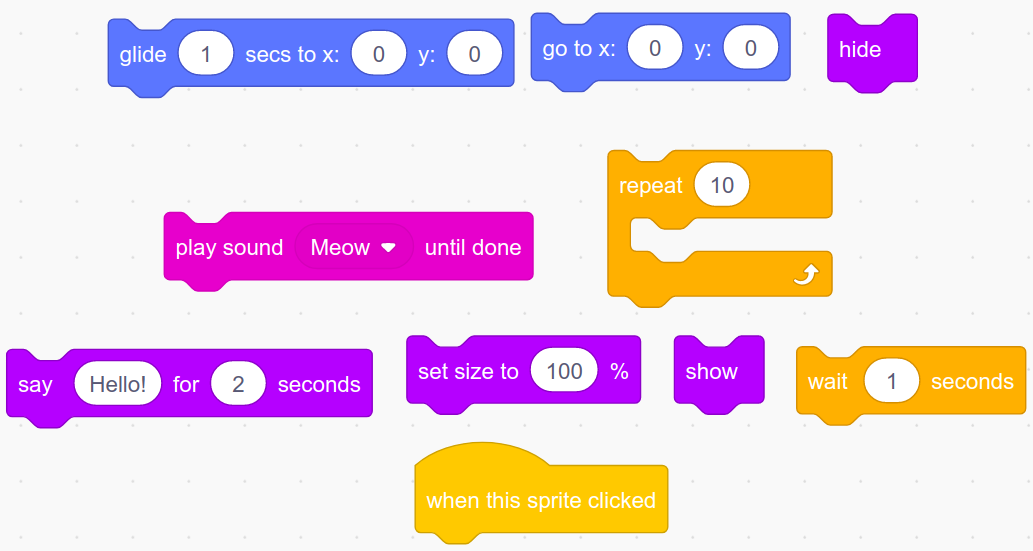
\includegraphics[width=0.9\linewidth]{figures/Scratch3.png}
  \caption{10 Scratch-blocks}
  \label{fig:blokke}
\end{figure}
Your task is to make a fun program only by using these blocks. Each
block may be used 0 or more times. Try first to connect the blocks on
paper, write down what you think the program will do and then create the
program in Scratch and run it. Describe to what extent the
program did as expected.
